\section{Results}
By combining the presented technology stacks, QNIBMonitoring provides deep insights into the complete cluster stack.

\subsection{Domain Modeling}
By using a schemaless graph database appraoch, each domain can be modeled independently. Common enteties are connected at any time after
they are modeled.

\subsubsection{Resource Scheduler}
\gls{slurm} provides information about resource allocations: Which jobs was started where, by whom at what time. How long did it last? What was the outcome? and alike.
The following \gls{slurm} entities are modeled as nodes within the graph.
\begin{description}
    \item[node] The SLURM node, which represents a compute node within the cluster, identified by the hostname.
    \item[partition] A logical group of nodes which represent the target of a job submission.
    \item[job] A demand for resources submitted by a user. Including metadata (user, submission/start/end time, job script, etc) and information about the state of the job.
        If resources are allocated, the job metadata is updated accordingly.
\end{description}
Relationships are added to connect certain nodes. $PART_OF$ indicates which a nodes membership to a partition. $JOBCLIENT$ connects a node to a certain running job.

\subsubsection{InfiniBand Interconnect}
An InfiniBand representation comprises of a set of physical and logical representations.
\begin{figure}[!ht]
    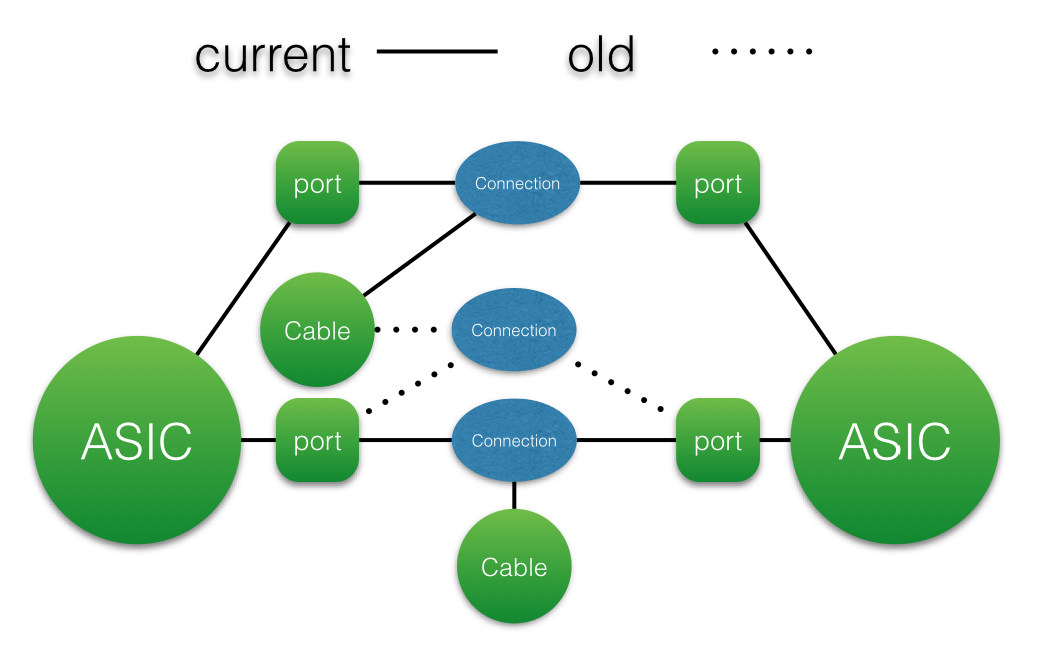
\includegraphics[width=.4\textwidth]{images/png/infiniband_graph.png}
    \caption{\label{fig:ib_graph}Modeling of an InfiniBand network.}
\end{figure}

\begin{description}
    \item[HCA] Network adapter pluged into a host/
    \item[SW] InfiniBand switch
    \item[PORT] Each $HCA$ and $SW$ are composed of a set of ports which provide connectivity.
    \item[CABLE] Physical connection between different ports.
    \item[CONNECTION] Logical entity which connects two $PORTS$ and a $CABLE$ for a given periode in time.
\end{description}


\subsection{Holistic Inventory}


\subsection{Open Log and Metric Framework}